\chapter{Deployment}\label{ch:deployment}
The deployment of the API Scout platform is divided into three main parts: databases, machine learning model, and web sever.
A general deployment structure can be found in Figure~\ref{fig:deployment-architecture}.
The databases run on two separate containers, one for the MongoDB instance, and one for the Elasticsearch instance.
The embedding machine learning model runs in a separate container, as does the web server.
All of these containers communicate together with a common Docker network, and only port 80 can be accessed from the outside.

\begin{figure}[h]
    \begin{center}
        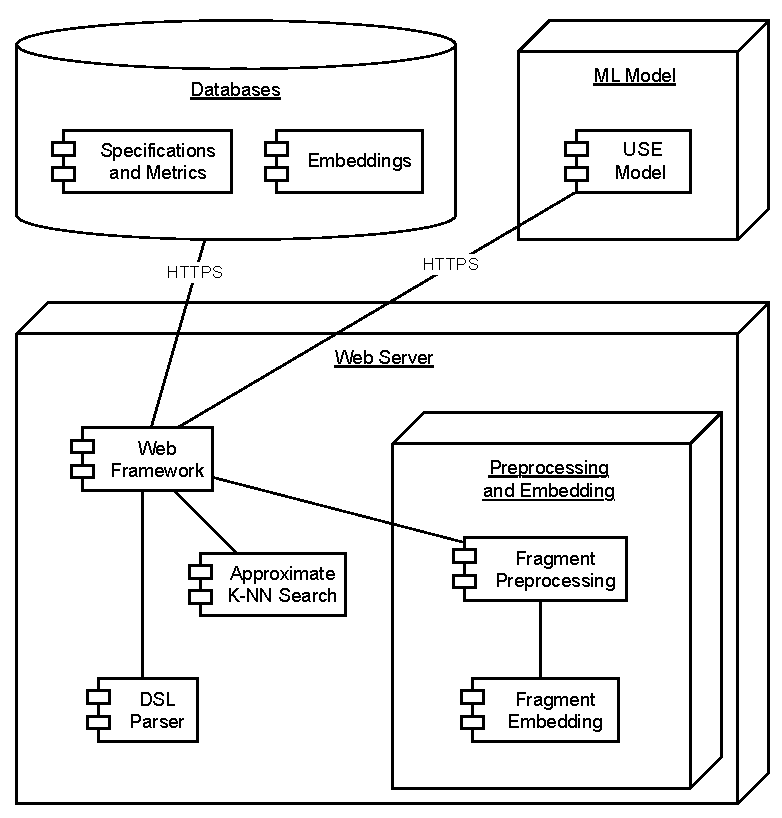
\includegraphics[width=0.55\linewidth]{assets/pdf/architecture/deployment-view}
    \end{center}

    \caption{API Scout's deployment architecture}
    \label{fig:deployment-architecture}
\end{figure}

\section{Databases}\label{sec:databases2}
The two databases -- MongoDB and Elasticsearch -- are contained in two separate Docker containers.
The Docker compose file for these two services is described in Listing~\ref{lst:compose-database}.
Both services do not expose any port to the outside, only in the \verb|backend| Docker network.
In addition, the Elasticsearch instance uses SSL/TLS to enable security when transporting data to and from the database.

\begin{lstlisting}[language=docker-compose,caption={Docker compose for the databases},label={lst:compose-database},captionpos=b]
version: "3.8"
services:
  mongo_db:
    container_name: mongo
    image: mongo:latest
    environment:
      "MONGO_INITDB_ROOT_USERNAME=root"
      "MONGO_INITDB_ROOT_PASSWORD=${MONGO_PASSWORD}"
    volumes:
      - "mongo:/data/db"
    networks:
      - backend

  es_db:
    container_name: es
    image: docker.elastic.co/elasticsearch/elasticsearch:8.12.2
    environment:
      - "node.name=es"
      - "cluster.initial_master_nodes=es"
      - "ELASTIC_PASSWORD=${ELASTIC_PASSWORD}"
      - "ES_JAVA_OPTS=-Xms6000m -Xmx6000m"
      - "xpack.license.self_generated.type=trial"
      - "xpack.security.enabled=true"
      - "xpack.security.http.ssl.enabled=true"
      - "xpack.security.http.ssl.key=${CERTS_DIR}/es/es.key"
      - "xpack.security.http.ssl.certificate_authorities=
          $CERTS_DIR/ca/ca.crt"
      - "xpack.security.http.ssl.certificate=$CERTS_DIR/es/es.crt"
      - "xpack.security.transport.ssl.enabled=true"
      - "xpack.security.transport.ssl.verification_mode=certificate"
      - "xpack.security.transport.ssl.certificate_authorities=
          ${CERTS_DIR}/ca/ca.crt"
      - "xpack.security.transport.ssl.certificate=${CERTS_DIR}/es/es.crt"
      - "xpack.security.transport.ssl.key=${CERTS_DIR}/es/es.key"
    volumes:
      - "data:/usr/share/elasticsearch/data"
      - "certs:${CERTS_DIR}"
    networks:
      - backend

  volumes: { "data", "certs", "mongo" }
  networks:
    backend:
      external: true
\end{lstlisting}

\section{ML Model}\label{sec:ml-model}
The machine learning model used for vector embedding (USE -- Section~\ref{subsec:document-embedding}) is served by a docker image called \verb|tensorflow/serving|.
This image expects a Tensorflow model to be inside the container.
Using this image, it creates several REST endpoints.
The endpoint used by us is the inference endpoint.
We pass a series of fragments as input, and the container will respond with their respective vector embeddings (as explained in Section~\ref{sec:use-model}).
The Docker compose file for this container is described in Listing~\ref{lst:compose-model}.

\begin{lstlisting}[language=docker-compose,caption={Docker compose for the ml model},label={lst:compose-model},captionpos=b]
      version: "3.8"
      services:
        models_ct:
          image: tensorflow/serving
          container_name: models
          environment:
           "MODEL_NAME=universal-encoder"
          volumes:
            - "./models/universal-encoder:/models/universal-encoder"
          networks:
            - backend

      networks:
        backend:
          external: true
\end{lstlisting}

\section{Web Server}\label{sec:web-server}
Finally, we have the Web server container.
This container is based off of a custom Docker image -- described in Listing~\ref{lst:dokerfile} -- in which we build both the Golang application, and the OpenAPI specification -- to create the web documentation for the service.

\begin{lstlisting}[language=docker,caption={Dockerfile for the web server},label={lst:dokerfile},captionpos=b]
           FROM golang:alpine as builder

           WORKDIR /backend

           COPY go.* ./
           RUN go mod download

           COPY . .
           RUN go install github.com/swaggo/swag/cmd/swag@latest
           RUN cd app && swag init
           RUN go build -o /backend/build/app /backend/app

           FROM alpine:latest

           WORKDIR /backend

           ARG GIN_MODE
           ARG MODELS_HOST

           COPY --from=builder /backend/build/app /backend/build/app

           EXPOSE 8080
           ENTRYPOINT [ "/backend/build/app" ]
\end{lstlisting}

\noindent After pushing the Docker image to Docker Hub, we pull it from the server and use the Docker compose document in Listing~\ref{lst:compose-web} to start the service.
Moreover, this is the only service that exposes a port outside the Docker network, namely, port 80.

\begin{lstlisting}[language=docker-compose,caption={Docker compose for the Web server},label={lst:compose-web},captionpos=b]
                   version: "3.8"
                   services:
                     web_server:
                       image: edoriggio/api-scout:dev
                       container_name: backend
                       environment:
                         "GIN_MODE=release"
                         "MODELS_HOST=models"
                       volumes:
                         - ./config:/backend/config
                         - ./ca.crt:/backend/ca.crt
                       networks:
                         - backend
                       ports:
                         - "8080:80"

                   networks:
                     backend:
                       external: true
\end{lstlisting}

\section{CI/CD pipeline}\label{sec:ci-cd-pipeline}
Regarding the Continuous Integration and Continuous Deployment (CI/CD) of the tool, we have implemented a pipeline for it in GitHub using GitHub Actions \footnote{https://docs.github.com/en/actions}.
GitHub Actions allows us to create YML files containing the pipeline we want GitHub to run whenever certain conditions are met.
Our pipeline is described in Listing~\ref{lst:ci-cd-pipeline}.
Now, we will analyze this file more in detail. \\ \\
As we can see at the top of the file (Lines 1--3), we have the name of the pipeline and the trigger.
The trigger, in this case, has been set to \verb|push|.
This means that every time a push event happens in GitHub in this specific repository, then the CI/CD pipeline will start.
Next, we have the jobs performed by the action (Lines 5--61). \\ \\
The first job to be performed is a testing job (Lines 6--32).
In this case, we check out the repo (Lines 9--10), set up the Golang environment (Lines 12--15), install of the dependencies present in the \verb|go.mod| file (Lines 17--20), build the application (Lines 22--23), run the tests using a special testing package (Lines 25--26), and finally export the test results as an artifact (Lines 28--32). \\ \\
The second and last job is a deployment job (Lines 34--61).
This job needs a few more conditions than the previous in order to run.
First of all, the testing pipeline must succeed for the deployment pipeline to run (Line 36).
Moreover, the job will run only if the push event is on either the \verb|main| or \verb|dev| branches.
This was done to avoid deploying unstable branches (Line 37).
Finally, we have the steps.
In this case, GitHub will checkout the repo (Lines 39--40), login into our Docker Hub \footnote{https://hub.docker.com/} account using some repository secrets (Lines 42--46), extract some metadata from the pull event (Lines 48--52), and finally build the Dockerfile and push the image to Docker Hub using the metadata to tag the image (Lines 54--61).

\begin{center}
    \lstset{
        numbers=left,
        firstnumber=1
    }

    \begin{lstlisting}[language=yaml,caption={YML file containing the CI/CD pipeline},label={lst:ci-cd-pipeline},captionpos=b]
      name: Test and Deploy Backend

      on: [ push ]

      jobs:
        test:
          runs-on: "ubuntu-latest"
          steps:
            - name: Checkout repo
              uses: actions/checkout@v4

            - name: Setup golang
              uses: actions/setup-go@v5
              with:
                go-version: "1.22"

            - name: Install dependencies
              run: |
                go install gotest.tools/gotestsum@latest
                go get ./...

            - name: Build
              run: go build -o ./main ./app

            - name: Run tests
              run: gotestsum ./app/tests/... > tests-result.txt

            - name: Upload tests result
              uses: actions/upload-artifact@v4
              with:
                name: tests-result
                path: tests-result.txt

        deploy:
          runs-on: ubuntu-latest
          needs: test
          if: contains("refs/heads/dev, refs/heads/main", github.ref)
          steps:
            - name: Checkout repo
              uses: actions/checkout@v4

            - name: Log in to Docker Hub
              uses: docker/login-action@v3
              with:
                username: ${{ secrets.DOCKER_USERNAME }}
                password: ${{ secrets.DOCKER_PASSWORD }}

            - name: Extract metadata
              id: meta
              uses: docker/metadata-action@v5
              with:
                images: edoriggio/api-scout

            - name: Build and push image
              uses: docker/build-push-action@v5
              with:
                context: .
                file: ./Dockerfile
                push: true
                tags: ${{ steps.meta.outputs.tags }}
                labels: ${{ steps.meta.outputs.labels }}
    \end{lstlisting}
\end{center}

\noindent Figure~\ref{fig:deployment-example} shows an example of a Docker image published to Docker Hub by our pipeline.
As we can see in this example, the image has been tagged \verb|:dev|.
This is because the pipeline was triggered on a push event on the \verb|dev| branch.
To pull the Docker image, one can run the command \verb|docker pull edoriggio/api-scou| \verb|t:dev|, or simply run \verb|docker-compose up -d| on the backend Docker compose file  (Section~\ref{sec:web-framework-1}).

\begin{figure}[h]
    \begin{center}
        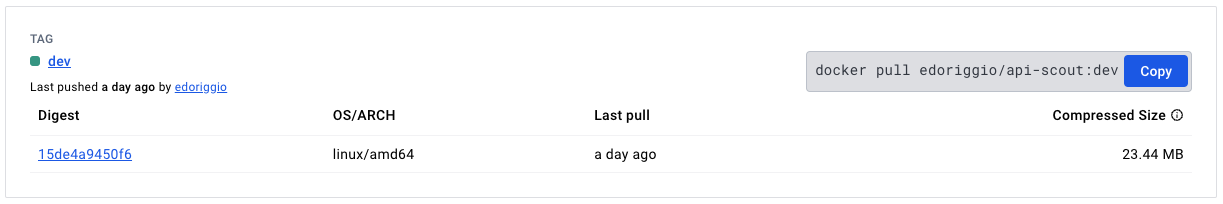
\includegraphics[width=0.9\linewidth]{assets/png/deployment/dev-deployment}
    \end{center}

    \caption{Example of a published Docker image}
    \label{fig:deployment-example}
\end{figure}
